\newif\ifdblatexpdf \ifx\pdfoutput\undefined \else \ifx\pdfoutput\relax \else\ifnum\pdfoutput>0 \dblatexpdftrue \fi \fi \fi
% ------------------------------------------------------------
% Autogenerated LaTeX file for books
% db2latex RELEASE: 0.8pre1
% db2latex VERSION: $Id: VERSION.xml,v 1.6 2004/01/31 12:47:11 j-devenish Exp $
% fithesis VERSION: 1.40
% ------------------------------------------------------------
\def\clsclass{rapport3}
\documentclass{fithesis}
% --------------------------------------------
% MetaFont and MetaPost logo support
% --------------------------------------------
\usepackage{mflogo}
% --------------------------------------------
% Load fithesis param 
% --------------------------------------------
\thesistitle{Real-time Communication in Web Browser}
\thesissubtitle{Master thesis}
\thesisstudent{Pavel Smolka}
\thesiswoman{false}
\thesislang{en}
\thesisyear{2013}
\thesisfaculty{fi}
\thesisadvisor{doc.
      RNDr. Tom� Pitner, Ph.D.}
% --------------------------------------------
\label{idp281040}% --------------------------------------------
% Load graphicx package with pdf if needed 
% --------------------------------------------
\ifdblatexpdf
\usepackage[pdftex]{graphicx}
\pdfcompresslevel=9
\else
\usepackage{graphicx}
\fi
\usepackage{anysize}
\marginsize{3cm}{2.5cm}{3.5cm}{3.5cm}

\makeatletter
% redefine the listoffigures and listoftables so that the name of the chapter
% is printed whenever there are figures or tables from that chapter. encourage
% pagebreak prior to the name of the chapter (discourage orphans).
\let\save@@chapter\@chapter
\let\save@@l@figure\l@figure
\let\the@l@figure@leader\relax
\def\@chapter[#1]#2{\save@@chapter[{#1}]{#2}%
\addtocontents{lof}{\protect\def\the@l@figure@leader{\protect\pagebreak[0]\protect\contentsline{chapter}{\protect\numberline{\thechapter}#1}{}{\thepage}}}%
\addtocontents{lot}{\protect\def\the@l@figure@leader{\protect\pagebreak[0]\protect\contentsline{chapter}{\protect\numberline{\thechapter}#1}{}{\thepage}}}%
}
\renewcommand*\l@figure{\the@l@figure@leader\let\the@l@figure@leader\relax\save@@l@figure}
\let\l@table\l@figure
\makeatother
\usepackage{fancyhdr}
\renewcommand{\headrulewidth}{0.4pt}
\renewcommand{\footrulewidth}{0.4pt}
% Safeguard against long headers.
\IfFileExists{truncate.sty}{
\usepackage{truncate}
% Use an ellipsis when text would be larger than x% of the text width.
% Preserve left/right text alignment using \hfill (works for English).
\fancyhead[ol]{\truncate{0.49\textwidth}{\sl\leftmark}}
\fancyhead[er]{\truncate{0.49\textwidth}{\hfill\sl\rightmark}}
\fancyhead[el]{\truncate{0.49\textwidth}{\sl\leftmark}}
\fancyhead[or]{\truncate{0.49\textwidth}{\hfill\sl\rightmark}}
}{\typeout{WARNING: truncate.sty wasn't available and functionality was skipped.}}
\pagestyle{fancy}
% ---------------------- 
% Most Common Packages   
% ---------------------- 
\usepackage{latexsym}         
\usepackage{enumerate}         
\usepackage{fancybox}      
\usepackage{float}       
\usepackage{ragged2e}       
\usepackage{fancyvrb}         
\makeatletter\@namedef{FV@fontfamily@default}{\def\FV@FontScanPrep{}\def\FV@FontFamily{}}\makeatother
\fvset{obeytabs=true,tabsize=3}
\makeatletter
\let\dblatex@center\center\let\dblatex@endcenter\endcenter
\def\dblatex@nolistI{\leftmargin\leftmargini\topsep\z@ \parsep\parskip \itemsep\z@}
\def\center{\let\@listi\dblatex@nolistI\@listi\dblatex@center\let\@listi\@listI\@listi}
\def\endcenter{\dblatex@endcenter}
\makeatother
\usepackage{rotating}         
\usepackage{subfigure}         
\usepackage{tabularx}         
\usepackage{url}         
% --------------------------------------------
% Load hyperref package with pdf if needed 
% --------------------------------------------
\ifdblatexpdf
\usepackage[pdftex,bookmarksnumbered,colorlinks,backref,bookmarks,breaklinks,linktocpage,plainpages=false, pdfstartview=FitH, plainpages=false, pdfpagelabels, unicode]{hyperref}
\else
\usepackage[bookmarksnumbered,colorlinks,backref,bookmarks,breaklinks,linktocpage,plainpages=false, plainpages=false, pdfpagelabels]{hyperref}
\fi
% --------------------------------------------
% ----------------------------------------------
% Define a new LaTeX environment (adminipage)
% ----------------------------------------------
\newenvironment{admminipage}%
{ % this code corresponds to the \begin{adminipage} command
 \begin{Sbox}%
 \begin{minipage}%
} %done
{ % this code corresponds to the \end{adminipage} command
 \end{minipage}
 \end{Sbox}
 \fbox{\TheSbox}
} %done
% ----------------------------------------------
% Define a new LaTeX length (admlength)
% ----------------------------------------------
\newlength{\admlength}
% ----------------------------------------------
% Define a new LaTeX environment (admonition)
% With 2 parameters:
% #1 The file (e.g. note.pdf)
% #2 The caption
% ----------------------------------------------
\newenvironment{admonition}[2] 
{ % this code corresponds to the \begin{admonition} command
 \hspace{0mm}\newline\hspace*\fill\newline
 \noindent
 \setlength{\fboxsep}{5pt}
 \setlength{\admlength}{\linewidth}
 \addtolength{\admlength}{-10\fboxsep}
 \addtolength{\admlength}{-10\fboxrule}
 \admminipage{\admlength}
 {\bfseries \sc\large{#2}} \newline
 \\[1mm]
 \sffamily
 \includegraphics[width=1cm]{#1}
 \addtolength{\admlength}{-1cm}
 \addtolength{\admlength}{-20pt}
 \begin{minipage}[lt]{\admlength}
 \parskip=0.5\baselineskip \advance\parskip by 0pt plus 2pt
} %done
{ % this code corresponds to the \end{admonition} command
 \vspace{5mm} 
 \end{minipage}
 \endadmminipage
 \vspace{.5em}
 \par
}
% --------------------------------------------
% Commands to manage/style/create floats      
% figures, tables, algorithms, examples, eqn  
% --------------------------------------------
 \floatstyle{plain}
 \restylefloat{figure}
 \floatstyle{plain}
 \restylefloat{table}
 \floatstyle{plain}
 \newfloat{program}{ht}{lop}[section]
 \floatstyle{plain}
 \newfloat{example}{ht}{loe}[section]
 \floatname{example}{Example}
 \floatstyle{plain}
 \newfloat{dbequation}{ht}{loe}[section]
 \floatname{dbequation}{Equation}
 \floatstyle{boxed}
 \newfloat{algorithm}{ht}{loa}[section]
 \floatname{algorithm}{Algorithm}
\ifdblatexpdf
\DeclareGraphicsExtensions{.pdf,.png,.jpg}
\else
\DeclareGraphicsExtensions{.eps}
\fi
% --------------------------------------------
% $latex.caption.swapskip enabled for $formal.title.placement support
\newlength{\docbooktolatextempskip}
\newcommand{\captionswapskip}{\setlength{\docbooktolatextempskip}{\abovecaptionskip}\setlength{\abovecaptionskip}{\belowcaptionskip}\setlength{\belowcaptionskip}{\docbooktolatextempskip}}
% Guard against a problem with old package versions.
\makeatletter
\AtBeginDocument{
\DeclareRobustCommand\ref{\@refstar}
\DeclareRobustCommand\pageref{\@pagerefstar}
}
\makeatother
% --------------------------------------------
\makeatletter
\newcommand{\dbz}{\penalty \z@}
\newcommand{\docbooktolatexpipe}{\ensuremath{|}\dbz}
\newskip\docbooktolatexoldparskip
\newcommand{\docbooktolatexnoparskip}{\docbooktolatexoldparskip=\parskip\parskip=0pt plus 1pt}
\newcommand{\docbooktolatexrestoreparskip}{\parskip=\docbooktolatexoldparskip}
\def\cleardoublepage{\clearpage\if@twoside \ifodd\c@page\else\hbox{}\thispagestyle{empty}\newpage\if@twocolumn\hbox{}\newpage\fi\fi\fi}
\usepackage[latin2]{inputenc}
\usepackage[T1]{fontenc}

\ifx\dblatex@chaptersmark\@undefined\def\dblatex@chaptersmark#1{\markboth{\MakeUppercase{#1}}{}}\fi
\let\save@makeschapterhead\@makeschapterhead
\def\dblatex@makeschapterhead#1{\vspace*{-80pt}\save@makeschapterhead{#1}}
\def\@makeschapterhead#1{\dblatex@makeschapterhead{#1}\dblatex@chaptersmark{#1}}

\AtBeginDocument{\ifx\refname\@undefined\let\docbooktolatexbibname\bibname\def\docbooktolatexbibnamex{\bibname}\else\let\docbooktolatexbibname\refname\def\docbooktolatexbibnamex{\refname}\fi}
% Facilitate use of \cite with \label
\newcommand{\docbooktolatexbibaux}[2]{%
  \protected@write\@auxout{}{\string\global\string\@namedef{docbooktolatexcite@#1}{#2}}
}
% Provide support for bibliography `subsection' environments with titles
\newenvironment{docbooktolatexbibliography}[3]{
   \begingroup
   \let\save@@chapter\chapter
   \let\save@@section\section
   \let\save@@@mkboth\@mkboth
   \let\save@@bibname\bibname
   \let\save@@refname\refname
   \let\@mkboth\@gobbletwo
   \def\@tempa{#3}
   \def\@tempb{}
   \ifx\@tempa\@tempb
      \let\chapter\@gobbletwo
      \let\section\@gobbletwo
      \let\bibname\relax
   \else
      \let\chapter#2
      \let\section#2
      \let\bibname\@tempa
   \fi
   \let\refname\bibname
   \begin{thebibliography}{#1}
}{
   \end{thebibliography}
   \let\chapter\save@@chapter
   \let\section\save@@section
   \let\@mkboth\save@@@mkboth
   \let\bibname\save@@bibname
   \let\refname\save@@refname
   \endgroup
}

%\usepackage{cite}
%\renewcommand\citeleft{(}  % parentheses around list
%\renewcommand\citeright{)} % parentheses around list
\newcommand{\docbooktolatexcite}[2]{%
  \@ifundefined{docbooktolatexcite@#1}%
  {\cite{#1}}%
  {\def\@docbooktolatextemp{#2}\ifx\@docbooktolatextemp\@empty%
   \cite{\@nameuse{docbooktolatexcite@#1}}%
   \else\cite[#2]{\@nameuse{docbooktolatexcite@#1}}%
   \fi%
  }%
}
\newcommand{\docbooktolatexbackcite}[1]{%
  \ifx\Hy@backout\@undefined\else%
    \@ifundefined{docbooktolatexcite@#1}{%
      % emit warning?
    }{%
      \ifBR@verbose%
        \PackageInfo{backref}{back cite \string`#1\string' as \string`\@nameuse{docbooktolatexcite@#1}\string'}%
      \fi%
      \Hy@backout{\@nameuse{docbooktolatexcite@#1}}%
    }%
  \fi%
}

% --------------------------------------------
% A way to honour <footnoteref>s
% Blame j-devenish (at) users.sourceforge.net
% In any other LaTeX context, this would probably go into a style file.
\newcommand{\docbooktolatexusefootnoteref}[1]{\@ifundefined{@fn@label@#1}%
  {\hbox{\@textsuperscript{\normalfont ?}}%
    \@latex@warning{Footnote label `#1' was not defined}}%
  {\@nameuse{@fn@label@#1}}}
\newcommand{\docbooktolatexmakefootnoteref}[1]{%
  \protected@write\@auxout{}%
    {\global\string\@namedef{@fn@label@#1}{\@makefnmark}}%
  \@namedef{@fn@label@#1}{\hbox{\@textsuperscript{\normalfont ?}}}%
  }

\makeindex
% index labeling helper
\newif\ifdocbooktolatexprintindex\docbooktolatexprintindextrue
\let\dbtolatex@@theindex\theindex
\let\dbtolatex@@endtheindex\endtheindex
\@ifundefined{@openrighttrue}{\newif\if@openright}{}
\def\theindex{\relax}
\def\endtheindex{\relax}
\newenvironment{dbtolatexindex}[2]
   {
\if@openright\cleardoublepage\else\clearpage\fi
\let\dbtolatex@@indexname\indexname
\def\dbtolatex@current@indexname{#2}
\ifx\dbtolatex@current@indexname\@empty                                                                                             \def\dbtolatex@current@indexname{\dbtolatex@@indexname}
\fi
\def\dbtolatex@indexlabel{%
 \ifnum \c@secnumdepth >\m@ne \ifx\c@chapter\undefined\refstepcounter{section}\else\refstepcounter{chapter}\fi\fi%
 \label{#1}\hypertarget{#1}{\dbtolatex@current@indexname}%
 \global\docbooktolatexprintindexfalse}
\def\indexname{\ifdocbooktolatexprintindex\dbtolatex@indexlabel\else\dbtolatex@current@indexname\fi}
\dbtolatex@@theindex
   }
   {
\dbtolatex@@endtheindex\let\indexname\dbtolatex@@indexname
   }

\newlength\saveparskip \newlength\saveparindent
\newlength\tempparskip \newlength\tempparindent

\def\docbooktolatexgobble{\expandafter\@gobble}
% Prevent multiple openings of the same aux file
% (happens when backref is used with multiple bibliography environments)
\ifx\AfterBeginDocument\undefined\let\AfterBeginDocument\AtBeginDocument\fi
\AfterBeginDocument{
   \let\latex@@starttoc\@starttoc
   \def\@starttoc#1{%
      \@ifundefined{docbooktolatex@aux#1}{%
         \global\@namedef{docbooktolatex@aux#1}{}%
         \latex@@starttoc{#1}%
      }{}
   }
}
% --------------------------------------------
% Hacks for honouring row/entry/@align
% (\hspace not effective when in paragraph mode)
% Naming convention for these macros is:
% 'docbooktolatex' 'align' {alignment-type} {position-within-entry}
% where r = right, l = left, c = centre
\newcommand{\docbooktolatex@align}[2]{\protect\ifvmode#1\else\ifx\LT@@tabarray\@undefined#2\else#1\fi\fi}
\newcommand{\docbooktolatexalignll}{\docbooktolatex@align{\raggedright}{}}
\newcommand{\docbooktolatexalignlr}{\docbooktolatex@align{}{\hspace*\fill}}
\newcommand{\docbooktolatexaligncl}{\docbooktolatex@align{\centering}{\hfill}}
\newcommand{\docbooktolatexaligncr}{\docbooktolatex@align{}{\hspace*\fill}}
\newcommand{\docbooktolatexalignrl}{\protect\ifvmode\raggedleft\else\hfill\fi}
\newcommand{\docbooktolatexalignrr}{}
\ifx\captionswapskip\@undefined\newcommand{\captionswapskip}{}\fi
\makeatother
\title{\bfseries Real-time Communication in Web Browser\\[12pt]\normalsize Master thesis}
\author{Pavel Smolka}
% --------------------------------------------
\makeglossary
% --------------------------------------------

\setcounter{tocdepth}{4}

\setcounter{secnumdepth}{4}
\begin{document}
% --------------------------------------------
% Useing fithesis
% --------------------------------------------
\FrontMatter
\ThesisTitlePage
\begin{ThesisDeclaration}
\DeclarationText
\AdvisorName
\end{ThesisDeclaration}

% --------------------------------------------
% Thanks 
% --------------------------------------------
\begin{ThesisThanks}
Thanks to everyone... TODO: Petr Kunc (help with OpenTok \& RealTime communication,\end{ThesisThanks}

% --------------------------------------------
% Abstract 
% --------------------------------------------
\begin{ThesisAbstract}

TODO
\end{ThesisAbstract}

% --------------------------------------------
% KeyWords 
% --------------------------------------------
\begin{ThesisKeyWords}
XMPP, real-time communication, RTC, Celebrio, web browser, HTTP, Comet, JavaScript, WebSockets, BOSH, TODO\end{ThesisKeyWords}

\makeatletter
\def\dbtolatex@contentsid{idp193696}
\def\dbtolatex@@contentsname{\latex@@contentsname}
\let\latex@@contentsname\contentsname
\newif\ifdocbooktolatexcontentsname\docbooktolatexcontentsnametrue
\def\dbtolatex@contentslabel{%
 \label{\dbtolatex@contentsid}\hypertarget{\dbtolatex@contentsid}{\dbtolatex@@contentsname}%
 \global\docbooktolatexcontentsnamefalse}
\def\contentsname{\ifdocbooktolatexcontentsname\dbtolatex@contentslabel\else\dbtolatex@@contentsname\fi}
\let\save@@@mkboth\@mkboth
\let\@mkboth\@gobbletwo
\tableofcontents
\let\@mkboth\save@@@mkboth
\let\contentsname\latex@@contentsname
\Hy@writebookmark{}{\dbtolatex@@contentsname}{\dbtolatex@contentsid}{0}{toc}%
\makeatother
				\MainMatter

% -------------------------------------------------------------
% Chapter Introduction 
% ------------------------------------------------------------- 	
\chapter{Introduction}
\label{uvod}\hypertarget{uvod}{}%

Millions, billions, trillions. That many and even more messages are exchanged every day between various people over the world. The Internet created brand new way to communicate and collaborate, even if you are located on the opposite parts of the world. Since the times of Alexander Graham Bell, the accesibility to the communication devices and their simplicity incredibly enhanced. Nowadays, almost 2.5 billion people over the world have access to the Internet and therefore they are able to use almost limitless communication possibilities it provides. \docbooktolatexcite{internet-usage}{}

However, the manner of Internet usage essentially changed during the first decade of 21st century. Using the Internet and using the web browser became almost synonyms. People use the web browser as the primary platform to do every single task on the Internet. Sometimes it's not even possible to use the other internet services without visiting certain web page in the web browser and performing the authentication there.\label{idp4831840}\begingroup\catcode`\#=12\footnote{
Two examples of such behavior. Wi-fi network in the Student Agency coaches forces the user to visit the entry page in the web browser. The second example, very well known to the students of the Faculty of Informatics at Masaryk University, is the faculty wireless network called wlan\_fi. Every user has to open the web browser and log in with her credentials. It's not possible just to open the terminal or e-mail client and start working online.
}\endgroup\docbooktolatexmakefootnoteref{idp4831840} Considering the mentioned fact, web browsers became also the basic platform for the communication tools. Even though the purpose of the world wide web and HTTP protocol was completely different at first (displaying single documents connected via hypertext links), it appeared that there is the need of common rich applications running withing web browser - rich internet application sprung up. \docbooktolatexcite{ria}{} So popular social networks are built on top of the web browser platform and they are used by more than billion people over the world. \docbooktolatexcite{facebook-usage}{} And the main reason why the social networks are so popular is the real-time stream of news and messages from the other people. By the beginning of the year 2013, I~would say that static web is dead - users prefer interactivity.

This thesis embraces the topic of real-time applications in web browsers, especially the text communication tools and the technologies being used to develop them. It also describes the problem of {``}inter-process{''} communication between various web pages which need to cooperate and exchange information as quickly as possible. Finally, the possibilities of multimedia content transfer (audio and video) and the current options of capturing multimedia directly from the web browser are described as well.

As mentioned above, the web browser became one of the most popular platforms. Celebrio, simple software for the elderly simulating the operating system interface, is typical example of rich internet application. \docbooktolatexcite{celebrio-system}{} All the topics mentioned in the previous paragraph appeared to be very important in the system. When interviewing the elderly people in the Czech Republic, it appeared that almost 90 \% of the elderly computer users use the real-time communication (RTC) applications, mostly Skype. \docbooktolatexcite{elderly-questionnaires}{} Interaction with their loved ones is the most desired benefit they expect from the computer. Therefore, creating real-time application, text messenger supporting video calling, became not only programming challenge but also a business goal.

Considering the fact the people like real-time communication (not only direct messaging but also real-time cooperation, simultaneous document editing or playing multiplayer games) while using web browser brings us the question what the currently available solutions are. There are {``}big players{''} providing their own services as closed-source, without the possibility to use them. To name the most important, it's Google Talk web browser client and Facebook chat, using XMPP protocol. \docbooktolatexcite{gtalk}{}\docbooktolatexcite{fb-chat}{} Even though Facebook chat service is not pure XMPP server implementation (the message and presence engine is proprietary system of Facebook implemented mostly in C++ and Erlang), they provide the possibility to connect to the {``}world of Facebook Chat{''} via XMPP as proxy. \docbooktolatexcite{fb-erlang}{} Combination of the facts that XMPP is open technology with open-sourced client and server implementations \docbooktolatexcite{xmpp-history}{} and the big internet companies also use it persuaded us to use it in our communication application too. XMPP itself and its usage in web applications is described in \hyperlink{chap-xmpp}{Chapter�{\ref{chap-xmpp}}, {``}Extensible Messaging and Presence Protocol{''}}.

Since the web browser was designed to perform simple requests/response interaction, it is not a typical platform for building real-time application. Thus, there is a need for an extra layer enhancing or even completely replacing the common way HTTP communicates. Within the scope of this thesis, namely the WebSockets and HTTP long polling approaches are used. The two of them and basic infromation about several others are covered in \hyperlink{chap-rtc}{Chapter�{\ref{chap-rtc}}, {``}Bidirectional communication{''}}.

There are many existing real-time chat-based applications over the Internet we could have used. However, none of them suited our needs perfectly. Celebrio has very specific graphical user interface (GUI) and there is a need to integrate both text-based chat and video calling. Just to mention, there is commercial chat module Cometchat\label{idp2608224}\begingroup\catcode`\#=12\footnote{
http://www.cometchat.com/
}\endgroup\docbooktolatexmakefootnoteref{idp2608224} or even open project Jappix.\label{idp2012608}\begingroup\catcode`\#=12\footnote{
https://project.jappix.com/
}\endgroup\docbooktolatexmakefootnoteref{idp2012608} Video calling web browser applications are provided for example by TokBox Inc.\label{idp3456192}\begingroup\catcode`\#=12\footnote{
http://www.tokbox.com/
}\endgroup\docbooktolatexmakefootnoteref{idp3456192} Nevertheless, following the rule that {``}If you have to customize 1/5 of a reusable component, its likely better to write it from scratch{''}, \docbooktolatexcite{brian-stats-tweet}{} just very generic existing libraries (Strophe.js) and APIs (OpenTok) were used for implementing brand new application called {\em{Celebrio Talker}}. The general approaches when building web browser based chat application are mentioned in \hyperlink{chap-xmpp-in-javascript}{Chapter�{\ref{chap-xmpp-in-javascript}}, {``}JavaScript XMPP client{''}}. Within the programming part of the thesis, the real-time text chat application, video calling application and simple {``}inter-process{''} communication tool for Celebrio has been implemented. Celebrio Talker application itself, its architecture and the specific procedures used to create it are described in \hyperlink{chap-talker}{Chapter�{\ref{chap-talker}}, {``}Talker{''}}.

It has been said that Skype\label{idp1416096}\begingroup\catcode`\#=12\footnote{
http://www.skype.com/
}\endgroup\docbooktolatexmakefootnoteref{idp1416096} is the most favorite communication tool among the target audience. If it had been implemented, the existing customer base could be used and converted to our messaging application. However, there is one big pitfall in this approach. Skype license strictly prohibits incorporating their software into mobile devices. \docbooktolatexcite{skype-license}{} They support only prompting the official Skype client to be opened via Skype URI, which is insufficient for Celebrio since the messaging client has to be built in the system, with the corresponding user interface. \docbooktolatexcite{skype-uri}{}

Finally, there are several notes about {``}inter-process communication{''} between different applications running separately in various browser frames, tabs or even windows. XrefId[??] covers this topic and describes the issues we came accross when implementing such functionality for Celebrio, where every application runs in separate iframe.

% -------------------------------------------------------------
% Chapter Bidirectional communication 
% ------------------------------------------------------------- 	
\chapter{Bidirectional communication}
\label{chap-rtc}\hypertarget{chap-rtc}{}%

The very essence of every instant messaging is the bidirectional stream where both sides can immediately {\em{push}} new data and the other side (or more other sides, respectively) is promptly notified without the need to perform any manual {\em{pull}} (update) action\index{pull \& push communication}.\label{idp4131344}\begingroup\catcode`\#=12\footnote{
In this thesis, this behaviour is commonly refered as RTC. The {``}real-time part{''} relates mostly to the server part since the application running in the web browser can perform the AJAX request on background anytime and the server receives the request instantly. Before AJAX became the essential part of every web app, ifram
}\endgroup\docbooktolatexmakefootnoteref{idp4131344} Such use case requires appropriate transport layer on top which the application can send the messages via any other protocol. When using HTTP, there is a TCP connection opened by the client (web browser) through which the data is sent. However, according to the HTTP protocol, the communication is strictly initiated by the client - HTTP is a request/response protocol. \docbooktolatexcite{rfc-http}{} When the client needs still up-to-date information, it must poll the server as frequently as possible. Such approach takes a lot of bandwidth and generates purposeless overhead on the server. So, when one wants to avoid that drawbacks and still make the web browser application to communicate in both directions, HTTP protocol must be hacked somehow or another communication channel has to be used. This chapter covers both - reshaping HTTP in \hyperlink{chap-http-requests}{Section�{\ref{chap-http-requests}}} and brand new approach in \hyperlink{chap-ws}{Section�{\ref{chap-ws}}}, bypassing HTTP at all. Unfortunatelly, every approach brings also some disadvantages.

% ------------------------   
% Section 
\section{Using HTTP requests}
\label{chap-http-requests}\hypertarget{chap-http-requests}{}%

Historicaly the first approach, for a very long time the only one, is hacking HTTP to achieve RTC. The idea is very simple. Generally, the client sends an extra request and it is not awaiting the response immediately. Instead, the server keeps the request for some time and sends the data as it comes in the response. There are several techniques to achieve such behaviour, in general called {\em{Comet}}\index{Comet}.

There is one common misunderstanding about long-lived HTTP requests. Since HTTP 1.1 (acutally implemented even before, but not covered in the RFC specification), there is a possibility for the client to claim persistent TCP connection to the server declaring {\texttt{{Connection: Keep-Alive}}} in the request header.\index{HTTP!Keep-Alive} Actually, all connections are considered persistent unless declared otherwise. \docbooktolatexcite{rfc-http}{} Even though the default timeout after which the server closes the connection is only a few seconds, \docbooktolatexcite{apache-core-features}{} the persistent TCP connection is very useful for delivering various resources (stylesheets, scripts, images, etc.) to the client without the unnecessary overhead of creating multiple streams. However, every single transmission within the TCP connection has to be in form of separate HTTP request/response, always initiated by the client. On no account is the server allowed to push any data without respective request from the client. Therefore, such TCP connection is of no use for RTC.

The situation is depicted at \hyperlink{fig-http-polling}{Figure�{\ref{fig-http-polling}}} and \hyperlink{fig-http-polling-wrong}{Figure�{\ref{fig-http-polling-wrong}}}. In the former case, a valid sequence of HTTP requests and responses is shown. Nevertheless, there is a delay between the moment the server gets (either generates or receives from third party) the data (2) and the following request (3). Yet it is possible to reduce the latency by shortening the polling time (the time between Response (1.1) and Request (3)), it is still trade-off between the delay and overhead caused by frequent empty request/response pairs.

% figure ------------------------------------------------------
\begin{figure}[hbt]
\hypertarget{fig-http-polling}{}%
\begin{center}

{{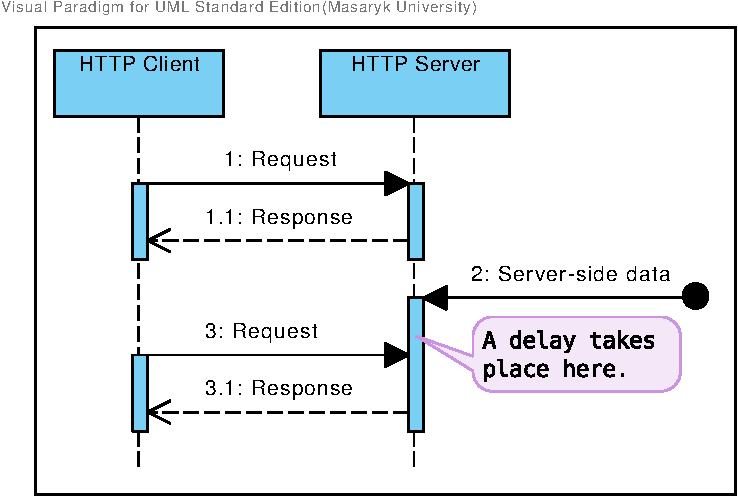
\includegraphics[]{vp/http-polling}}\hypertarget{idp160336}{}%
\label{idp160336}
}
{{\caption[{Correct HTTP polling with delay}]{{{Correct HTTP polling with delay}}}\label{fig-http-polling}}}
\end{center}
\end{figure}

% figure ------------------------------------------------------
\begin{figure}[hbt]
\hypertarget{fig-http-polling-wrong}{}%
\begin{center}

{{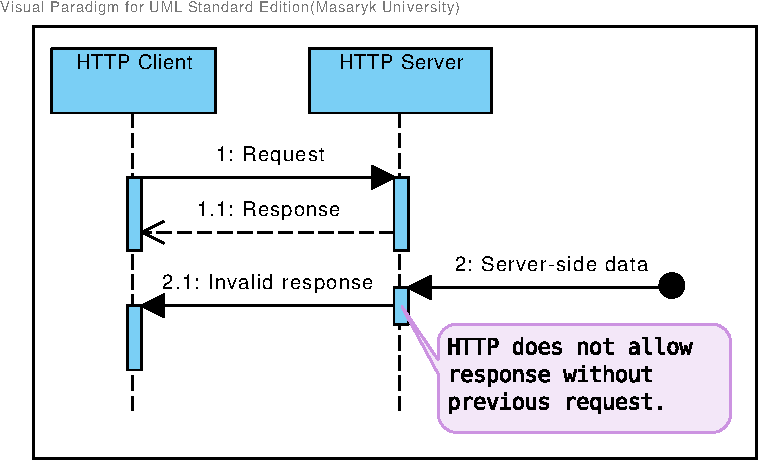
\includegraphics[]{vp/http-polling-wrong}}\hypertarget{idp163024}{}%
\label{idp163024}
}
{{\caption[{Forbidden HTTP response without respective request}]{{{Forbidden HTTP response without respective request}}}\label{fig-http-polling-wrong}}}
\end{center}
\end{figure}

On the other hand, \hyperlink{fig-http-polling-wrong}{Figure�{\ref{fig-http-polling-wrong}}} depicts the forbidden situation of generating HTTP response without request immediately. When the server gets the data (2) it is not allowed to initiate the connection and send HTTP response without appropriate preceding request (2.1). Even though the delay, mentioned in the previous paragraph, can be minimized in this situation, HTTP servers cannot use such technique. To sum it up, response (2.1) is forbidden by HTTP protocol and this situation solution is not valid.
\subsection{HTTP long polling\index{HTTP!long polling}}
\label{chap-http-long-polling}\hypertarget{chap-http-long-polling}{}%

The essence of HTTP long polling springs from the idea of prolonging the time span between two poll requests. In traditional {``}short polling{''}, a client sends regular requests to the server and each request attempts to {``}pull{''} the available data. If no data is available, an empty reponse is sent. \docbooktolatexcite{rfc-bidirectional-http}{} That generates unnecessary overhead for both client and server.

On the contrary, long polling tries to reduce this load. After receiving the request, the server {\em{does not}} answer immediately and holds the connection opened. When the server receives (or even makes up by itself) new data, it carries out the response with the respective content, as depicted at \hyperlink{fig-http-long-polling}{Figure�{\ref{fig-http-long-polling}}}.

% figure ------------------------------------------------------
\begin{figure}[hbt]
\hypertarget{fig-http-long-polling}{}%
\begin{center}

{{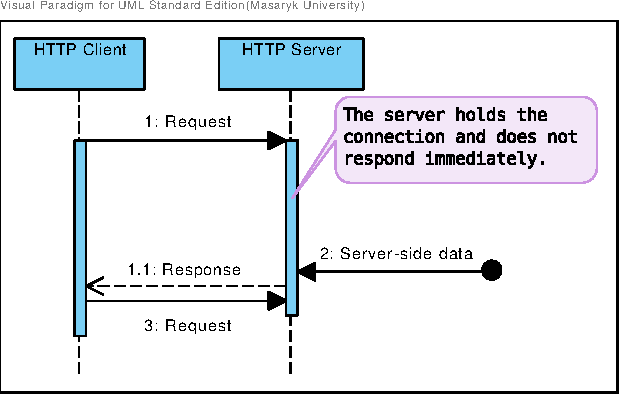
\includegraphics[]{vp/http-long-polling}}\hypertarget{idp5485968}{}%
\label{idp5485968}
}
{{\caption[{HTTP long polling}]{{{HTTP long polling}}}\label{fig-http-long-polling}}}
\end{center}
\end{figure}

As soon the client obtains the response, it usually issues a new request immediately so the process can repeat endlessly. If no data appears on the server for certain amount of time, it usually responds with empty data field just to renew the connection.

One of the main drawbacks of long polling is header overhead. Every chunk of data in RTC applications is usually very short, for example some text message of minimal length. However, each update is served by full HTTP request/response with the header easily reaching 800 characters. \docbooktolatexcite{pro-html5-programming}{} In case the payload is a message 20 characters long, the header constitutes 4000\% overhead!\index{HTTP!header overhead} This drawback has even bigger impact as the number of clients increases. \hyperlink{fig-http-overhead}{Figure�{\ref{fig-http-overhead}}} shows the comparsion of 1000 (A), 10000 (B) and 100000 (C) clients polling the server every second with the message 20 characters long, both using classic HTTP requests and WebSockets technology (mentioned in \hyperlink{chap-ws}{Section�{\ref{chap-ws}}}). \docbooktolatexcite{pro-html5-programming}{}

% figure ------------------------------------------------------
\begin{figure}[hbt]
\hypertarget{fig-http-overhead}{}%
\begin{center}

{{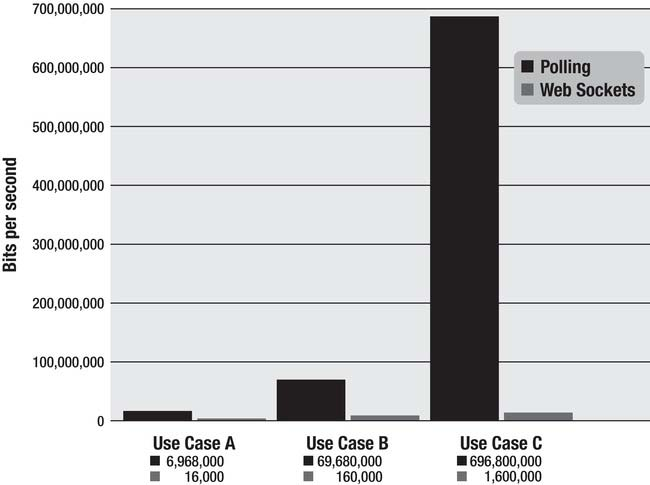
\includegraphics[width=420pt]{img/http-overhead}}\hypertarget{idp5493760}{}%
\label{idp5493760}
}
{{\caption[{Comparison of the unnecessary network overhead between the HTTP polling and using WebSockets \docbooktolatexcite{pro-html5-programming}{}}]{{{Comparison of the unnecessary network overhead between the HTTP polling and using WebSockets \docbooktolatexcite{pro-html5-programming}{}}}}\label{fig-http-overhead}}}
\end{center}
\end{figure}

Furthermore, in case the server just received the data and sent the response to the client, there is a {``}blind window{''} when the server cannot notify the client. Whole push system is blocked until the response is received by the client, processed and new request is delivered back to the server. Considering also the possible packet loss and required retransmission in TCP protocol, the delay can be even longer than double bandwidth latency. \docbooktolatexcite{rfc-bidirectional-http}{}
\subsection{HTTP streaming\index{HTTP!streaming}}
\label{chap-http-streaming}\hypertarget{chap-http-streaming}{}%

HTTP streaming is slightly different technique than long polling, although they are confused one with the other very often. What is mutual for both of the approaches is the client initializing the communication by HTTP request. The server also sends the update as the part of the HTTP response. The main difference is that once the server initializes the response and sends the data, it does not terminate the response and keeps the HTTP connection opened. Meanwhile, the client listens to the response stream and reads the data pushed from the server. When any new data springs up on the server side, it is concatenated to the one existing response stream. \docbooktolatexcite{rfc-bidirectional-http}{} See the schema at \hyperlink{fig-http-streaming}{Figure�{\ref{fig-http-streaming}}}.

% figure ------------------------------------------------------
\begin{figure}[hbt]
\hypertarget{fig-http-streaming}{}%
\begin{center}

{{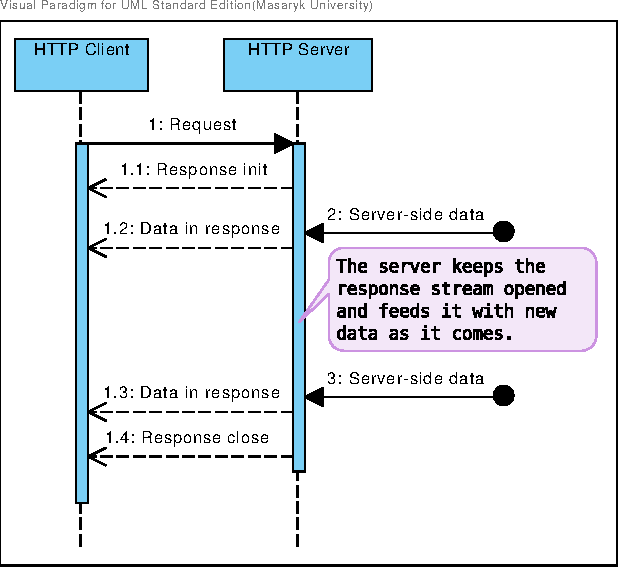
\includegraphics[]{vp/http-streaming}}\hypertarget{idp5503072}{}%
\label{idp5503072}
}
{{\caption[{HTTP streaming}]{{{HTTP streaming}}}\label{fig-http-streaming}}}
\end{center}
\end{figure}

It is very important not to confuse HTTP streaming with the {``}persistent{''} HTTP requests. As said at the beginning of this chapter, declaring {\texttt{{Connection: Keep-Alive}}} does not allow the server to issue multiple responses to a single request. Such behaviour would be serious violation of HTTP protocol. Instead, the server can declare {\texttt{{Transfer-Encoding: chunked}}}\index{HTTP!chunked response} status in the response header and send the response split into separate pieces, as show below (chunk of zero length stands for the end of the response): \docbooktolatexcite{rfc-bidirectional-http}{}

\begin{Verbatim}[fontsize=\small]
HTTP/1.1 200 OK
Content-Type: text/plain
Transfer-Encoding: chunked

25
This is the data in the first chunk

1C
and this is the second one

0
\end{Verbatim}

The main drawback of HTTP streaming can be generally called buffering. There is no requirement for both the client and any intermediary (proxies, gateways, etc.) to handle the incoming data until whole response is sent. Therefore, all parts of the response could be kept by the proxy and the messages (single HTTP response chunks) are not delivered to the client until whole response is sent. Similarly, when the response consists of JavaScript statements, the browser does not have to execute them before whole response is obtained (yet, most of the browsers execute it immediately). In such cases, HTTP streaming will not work. \docbooktolatexcite{rfc-bidirectional-http}{}

% ------------------------   
% Section 
\section{WebSockets}
\label{chap-ws}\hypertarget{chap-ws}{}%

Although the World Wide Web with HTTP request/response schema has never been intended to server as RTC platform, the contemporary applications require such functionality and the developers started to bend the protocol in the undesirable way. Most of the patterns described in \hyperlink{chap-http-streaming}{Section�{\ref{chap-http-streaming}}} do their jobs and one can achieve sufficient two-way communication, but there are certain performance issues and drawbacks which make them difficult to use. At least, those techniques carry HTTP header overhead which is unnecessary for standard bidirectional streams. Therefore, brand new standard for creating full-duplex communication channels between the web browser and the server has been created. The technology is called {\em{WebSockets}}\index{WebSocket} (sometimes shortened as WS) and it stands for a communication protocol layered over TCP along with the browser API for web developers. Anyway, not even WebSockets are allowed to access wider network, the connection possibilities are limited only to the dedicated WS servers (usually HTTP servers with additional module for WS support attached). \docbooktolatexcite{js-definitive-guide}{}

Similarly as in HTTP, there is an unencrypted version of WebSockets working directly on top of TCP connection. The simpliest way to recognize such connection is WebSocket URI\index{WebSocket!URI} beginning with {\texttt{{ws://}}}. It should not be used on account of two reasons. The first one, quite obvious, is security - the communication can be captured during the transmission. Transparent proxy servers are the second reason. If an unencrypted WebSocket connection is used, the browser is unaware of the transparent proxy and as a result, the WebSocket connection is most likely to fail. \docbooktolatexcite{ws-proxy}{}\docbooktolatexcite{definitive-guide-to-ws}{} As opposite, there is a secure way how to use WebSockets. WebSockets Secure (WSS)\index{WebSocket!Secure} protocol is standard WS wrapped in TLS tunnel, similarly as HTTP can be transmitted over TLS layer. When using WSS, the URI begins with {\texttt{{wss://}}} and it uses port 443 by default. \docbooktolatexcite{definitive-guide-to-ws}{}
\subsection{Handshake\index{WebSocket!handshake}}
\label{idp5521696}\hypertarget{idp5521696}{}%

Alike any other multilateral protocol WebSockets need to perform a handshake before actual transmission can take place. During the handshake, the connection is established and both peers acknowledge the properties of the communication.

Since WebSockets emerged as HTTP supplement, the handshake is initialized by HTTP request\label{idp5524624}\begingroup\catcode`\#=12\footnote{
According to RFC6455, the protocol is designed to work over HTTP ports 80 and 443 as well to support HTTP proxies. However, the design is not limited to HTTP and the future implementations can use simplier handshake over a dedicated port. \docbooktolatexcite{rfc-ws}{}
}\endgroup\docbooktolatexmakefootnoteref{idp5524624} initialized by the client. The client sends the request as follows: \docbooktolatexcite{rfc-ws}{}

\begin{Verbatim}[fontsize=\small]
GET /chat HTTP/1.1
Host: server.example.com
Upgrade: websocket
Connection: Upgrade
Sec-WebSocket-Key: dGhlIHNhbXBsZSBub25jZQ==
Origin: http://example.com
Sec-WebSocket-Protocol: chat, superchat
Sec-WebSocket-Version: 13
\end{Verbatim}

Let us have a look what each of the lines means. The first two lines are obvious, they represent typical HTTP GET request. Specifying {\texttt{{Host}}} is important for the server to be able to handle multiple virtual hosts on single IP address. The following two lines, {\texttt{{Upgrade: websocket}}} and {\texttt{{Connection: Upgrade}}}, are the most important. The client informs the server about the desire to use WS. The rest of the request stands for additional information for the server to be able to respond correctly - RFC 6455 describes them in detail.

The server should send HTTP response looking similar as this example: \docbooktolatexcite{rfc-ws}{}

\begin{Verbatim}[fontsize=\small]
HTTP/1.1 101 Switching Protocols
Upgrade: websocket
Connection: Upgrade
Sec-WebSocket-Accept: s3pPLMBiTxaQ9kYGzzhZRbK+xOo=
\end{Verbatim}

Number 101 on the first line of the response stands for HTTP status code {\texttt{{Switching Protocols}}}, \docbooktolatexcite{rfc-http}{} which means the server supports WebSockets and the connection can be established. Any status code other than 101 indicates that the WebSocket handshake has not completed and that the semantics of HTTP still apply. \docbooktolatexcite{rfc-ws}{}

{\texttt{{Sec-WebSocket-Key}}} is random secret issued by the client and added to the initial protocol-switching request. The server is supposed to concatenate the secret with Globally Unique Identifier (GUID)\index{GUID} "258EAFA5-E914-47DA- 95CA-C5AB0DC85B11" and hash the result with SHA-1 algorithm. The resultis returned as {\texttt{{Sec-WebSocket-Accept}}} header field, base64-encoded. \docbooktolatexcite{rfc-ws}{} However, there seems to be a security issue here. If the initial request is not sent over encrypted HTTP connection (HTTPS), it can be caught by a third party. Since the server does not authenticate in any way and the algorithm does not contain any server secret, the third party attacker could fake the response and pretend to be the server.
\subsection{Frames and masking}
\label{idp5537440}\hypertarget{idp5537440}{}%

All the data sent via WebSockets protocol is chunked into frames\index{frames}, working similarly as TCP frames. All the transmission features are handled by the WebSocket API and the transmission is transparent for the application layer above (for example JavaScript API) so that that every message appears in the same state as it was sent. This means the message, single portion of WS communication, can be fragmented during the transmission.

There are several special features concerning WS frames, one of the interesting is masking\index{masking}. The payload data of every frame sent from the client is XORed by the masking key of 32-bit size. The purpose of masking is to prevent any third party from picking any part of the payload and reading it. The other goal might be distinguishing the server stream from the client stream instantly since client-to-server frames always {\em{must}} be masked and server-to-client frames {\em{must not}} be masked under any circumstances. In addition, WS peers have to use masking even if the communication is running on top of TLS layer so the {``}encryption{''} function is pointless. \docbooktolatexcite{rfc-ws}{} The security function of masking is also questionable because the masking key is included in the frame header. The only reason is preventing from random cross-protocol attacks. \docbooktolatexcite{pro-html5-programming}{}
\subsection{JavaScript API\index{WebSocket!API}}
\label{idp5544192}\hypertarget{idp5544192}{}%

Since WebSocket technology is intended to be used particularly from the browser applications, there is need of an API web developers can use. The most widespread programming language of web browser client applications is JavaScript and so is the WebSocket API created for. The API consists of one relatively simple JavaScript interface called {\texttt{{WebSocket}}},\label{idp5547376}\begingroup\catcode`\#=12\footnote{
In the older versions of some browsers, the interface was called differently due to the immaturity of the technology. For instance, Firefox from version 6 to 10 supports WebSockets only as {\texttt{{MozWebSocket}}}. Interesting fact is that Firefox 4 and 5 provides {\texttt{{WebSocket}}} interface as it is, just implementing different WebSocket protocol version. Since Firefox 11.0, current (RFC 6455) WS protocol version is accessible via interface {\texttt{{WebSocket}}}. \docbooktolatexcite{mozilla-ws}{}
}\endgroup\docbooktolatexmakefootnoteref{idp5547376} \docbooktolatexcite{ws-api}{} placed as the property of {\texttt{{window}}} object.\label{idp5551840}\begingroup\catcode`\#=12\footnote{
Properties of window are accessible in JavaScript directly. Simple test {\texttt{{window.WebSocket === WebSocket}}} returning {\texttt{{true}}} proves it.
}\endgroup\docbooktolatexmakefootnoteref{idp5551840} It wraps the WebSocket client functionality performed by the user agent (web browser). Using the API is very simple - the object, which handles all the WS functionality, is created by calling {\texttt{{WebSocket()}}} constructor: \docbooktolatexcite{ws-html5rocks}{}

\begin{Verbatim}[fontsize=\small]
var connection = new WebSocket(
        'ws://html5rocks.websocket.org/echo', 
        ['soap', 'xmpp']
);
\end{Verbatim}

The first (mandatory) argument stands for the WebSocket URI the client attempts to connect to. It can either begin with ws:// prefix or wss://, depending whether TLS layer is used or not. The second parameter is optional - specific WS subprotocols can be demanded there. Since there are only a few subprotocols recorded by IANA registry, it is of a little use so far. \docbooktolatexcite{ws-iana}{}

{\texttt{{WebSocket}}} interface provides at least four event handlers, to each of them a custom callback can be attached. \docbooktolatexcite{ws-api}{} Those are {\texttt{{onopen}}}, {\texttt{{onmessage}}}, {\texttt{{onerror}}} and {\texttt{{onclose}}}. The names are quite self-explanatory, they serve as the event listeners watching the incoming activity - anytime the websocket obtains a message, its status changes or an error occurs, the respective callback is fired. The callback registration can look as follows:

\begin{Verbatim}[fontsize=\small]
connection.onmessage = function (message) {
  console.log('We got a message: ' + message.data);
};
\end{Verbatim}

In addition, there is a property {\texttt{{readyState}}} (it would be {\texttt{{connection.readyState}}} in the previous example) keeping current WebSocket status all the time. The status can be retrieved by testing the property against one of the {\texttt{{WebSocket}}} property constants {\texttt{{CONNECTING}}}, {\texttt{{OPEN}}}, {\texttt{{CLOSING}}} or {\texttt{{CLOSED}}}.

Sending the data to the server is also quite straightforward. Either {\texttt{{DOMString}}}, {\texttt{{ArrayBuffer}}}, {\texttt{{ArrayBufferView}}} or {\texttt{{Blob}}} can be sent via {\texttt{{send()}}} method. See the examples below: \docbooktolatexcite{ws-html5rocks}{}

\begin{Verbatim}[fontsize=\small]
// Sending String
connection.send('string message');

// Sending canvas ImageData as ArrayBuffer
var img = canvas_context.getImageData(0, 0, 400, 320);
var binary = new Uint8Array(img.data.length);
for (var i = 0; i < img.data.length; i++) {
  binary[i] = img.data[i];
}
connection.send(binary.buffer);

// Sending file as Blob
var file = document.querySelector('input[type="file"]').files[0];
connection.send(file);
\end{Verbatim}

To sum it up, using WebSockets became a very simple and elegant way to provide real-time communication channel between web browser and WS server. The main drawback of WS is lack of support not only in the older versions of web browsers but also in the mobile platform browsers. Currently less than 60 \% of users can make use of WebSocket full support. \docbooktolatexcite{ws-caniuse}{} Particularly, all versions of Internet Explorer below 10 (which means more than 98 \% of IE users in November 2012) \docbooktolatexcite{ie-statistics}{} does not implement WebSockets JavaScript API. There are two favourable aspects in favour of WebSockets. Firstly, more and more web browsers add JavaScript API to support WebSockets. Secondly, the ratio of clients who use old version of the web browser without WS support tends to diminish. Anyway, if the real-time functionality constitutes the application core functionality, there is a strong need to offer fallback technology that every browser supports - usually represented by HTTP long polling or streaming mechanism, described in \hyperlink{chap-http-requests}{Section�{\ref{chap-http-requests}}}.

% ------------------------   
% Section 
\section{High-level RTC frameworks}
\label{idp5575696}\hypertarget{idp5575696}{}%

Actually, there are several higher level solutions for achieving bidirectional (and thus real-time) communication in web browser. Some of them use HTTP requests described above (such as Bayeux), some of them are based on WebSockets (WebRTC) and several are built completely independent, installed as web browser plugins and thus behaving like separate runtime platforms (Adobe Flash).
\subsection{Adobe Flash}
\label{idp5577152}\hypertarget{idp5577152}{}%

Among all, one of the most widespread technologies is Adobe Flash.\label{idp5578144}\begingroup\catcode`\#=12\footnote{
http://www.adobe.com/software/flash/about/
}\endgroup\docbooktolatexmakefootnoteref{idp5578144} Apart from the possibility to establish bidirectional persistent TCP connection, Flash allows the developer to create almost any graphics, animations and user interface with nearly no limits.

Nevertheless, the disadvantages of Flash are significat. First, Flash is not a native part of any web browser. Until recently, it had to be installed manually as a plugin. Now, it is bundled and shipped with Chromium-based browsers (Chrome, Chromium), but it is still external plugin. \docbooktolatexcite{flash-bundled-with-chrome}{} Another drawback of Flash is lack of support on mobile devices. Apple has been clear about it: iPhones and iPads have never supported Flash technology and it is not likely to change in the future. \docbooktolatexcite{iphone-flash-support}{} Android devices supported Flash at first, but later Adobe quit Google Play. \docbooktolatexcite{android-flash-support}{}

There are many other similar technologies such as Adobe Flash, but they all suffer the same pain. Since they are installed as proprietary plugins, the developer can never be sure the application will run in any environment. This concerns technologies like Microsoft Silverlight\label{idp5581952}\begingroup\catcode`\#=12\footnote{
http://www.microsoft.com/silverlight/
}\endgroup\docbooktolatexmakefootnoteref{idp5581952} or Adobe AIR\label{idp5582720}\begingroup\catcode`\#=12\footnote{
http://www.adobe.com/products/air.html
}\endgroup\docbooktolatexmakefootnoteref{idp5582720} (even though AIR has been intended to be browser-independent platform).

So, Adobe Flash is often used as a fallback for older browsers, running on non-mobile devices, which does not WebRTC yet (described below). It has been used as fallback for the video calls in Talker application. However, creating a new application based on Flash (as a primary technology) in 2013 is not a good idea.
\subsection{WebRTC}
\label{idp5584944}\hypertarget{idp5584944}{}%

WebRTC (http://www.webrtc.org/)
\subsection{Other frameworks}
\label{idp5586096}\hypertarget{idp5586096}{}%

Bayeux: http://svn.cometd.org/trunk/bayeux/bayeux.html

OpenTok

SignalR (.NET)

Google hangouts API

% -------------------------------------------------------------
% Chapter Extensible Messaging and Presence Protocol 
% ------------------------------------------------------------- 	
\chapter{Extensible Messaging and Presence Protocol}
\label{chap-xmpp}\hypertarget{chap-xmpp}{}%

Extensible Messaging and Presence Protocol (XMPP) technologies were invented by Jeremie Miller in 1998. \docbooktolatexcite{xmpp-the-definitive-guide}{} It is one of the most widespread technologies for instant messaging (IM),\label{idp5590400}\begingroup\catcode`\#=12\footnote{
Acutally, the IM client or even the techology itself is sometimes called {``}Instant Messenger{''}. This term is registered as a trademark by AOL company. \docbooktolatexcite{aol-trademarks}{}
}\endgroup\docbooktolatexmakefootnoteref{idp5590400} i.e. exchanging the text or multimedia data between several endpoints. The {``}native{''} implementation of XMPP works right on top of TCP protocol: XMPP endpoint (called client as it represents the first actor in client-server architecture) opens long-lived TCP connection. Then, both the client and the server negotiate and open XML streams so there is one stream in each direction. \docbooktolatexcite{xmpp-the-definitive-guide}{} When the connection is established, both client and server can push any changes as XML elements to the stream and the other side obtains them immediately. Usual XMPP clients are standalone applications able to open TCP connection and listen to the stream opened by the server.

XMPP stands for communication protocol handling not only sending and receiving the messages, but also presence notification, contact list (roster) management and others. The architecture is distributed and decentralized. There is no central or top level XMPP server. Anyone can run XMPP server, very similarly as HTTP or FTP server. Identification and recognition on the network is also similar - XMPP relies on Domain Name System (DNS) so that every server is identified via string domain name with arbitrary subdomain level (e.g. xmpp.example.com or just example.org). \docbooktolatexcite{xmpp-the-definitive-guide}{}

The user names have the same structure as e-mail addresses so the user name is followed by at sign and the server domain name. This rule also guarantees that every XMPP user is registered at the certain server. If there is any message or notification for the given user, her {``}home{''} server is looked up first, the message is transferred to that server first and then, the respective server (that the user belongs to) is responsible for delivering the message to the user or saving it until the user logs in. Therefore, two possible connection types take place in XMPP. Client-to-server communication is the first one, when the clients can talk only to their {``}home{''} server. Then, server-to-server communication is designed for delivering the messages to the users at different domains. When two servers are exchanging any data, direct connection to the target server is established. This approach is dissimilar to the way SMTP servers exchange e-mail messages. It helps to prevent address spoofing or spamming. \docbooktolatexcite{xmpp-the-definitive-guide}{}

XMPP has been chosen as the communication protocol for this thesis topic - Talker application. XMPP has been verified by big companies such as Google or Facebook. In addition, the openness of the protocol allows very easy connection to existing wide communication networks, using their server infrastructure, client software and existing user base.

% ------------------------   
% Section 
\section{XML Stanzas}
\label{chap-xmpp-stanzas}\hypertarget{chap-xmpp-stanzas}{}%

As mentioned in the introduction to this chapter, when XMPP connection is established, two streams are opened and both the client and the server can send any XML elements at any time. The meanings of various pieces of XML are described in this section.

There are three three basic XML elements that every XMPP communication consists of. Those are {\texttt{{\textless{}message/\textgreater{}}}}, {\texttt{{\textless{}presence/\textgreater{}}}} and {\texttt{{\textless{}iq/\textgreater{}}}} (which stands for Info/Query), altogether called {\texttt{{Stanza}}}\index{stanza}s. \docbooktolatexcite{xmpp-the-definitive-guide}{} Each stanza element usually contains several attributes which specify the exact meaning of it. The actual content is usually placed in the element body. Example message\index{XMPP!message} stanza can look like this:

\begin{Verbatim}[fontsize=\small]
<message from="pavel.smolka@celebrio.cz/talker"
         to="tomas.pitner@celebrio.cz"
         type="chat">
    <body>Hello, how are you?</body>
</message>
\end{Verbatim}

The attributes {\texttt{{from}}} and {\texttt{{to}}} stand for the sender and recipient of the message. Actually, the value the sender sets to the {\texttt{{from}}} attribute (or whether she entirely leaves it out) does not matter. The {``}home{''} XMPP server the sender is registered at (in this example, it would be the one running at {\texttt{{celebrio.cz}}}) has to set the from attribute according to the real user name and domain name. This is one of the interesting defensive mechanisms distinguishing XMPP from other communication protocols as SMTP.

You might have noticed that {\texttt{{from}}} field does not contain only the XMPP address. There is a {\em{resource}}\index{XMPP!resource} identifier after the domain name. Since it is possible to connect multiple times with the same user name, the resource makes a difference between the sessions of the same user. In addition, it is useful information for other peers the user might communicate with. It is usual to set the resource field according to the place the user logs from or the device she uses.

Message stanza receiving is not acknowledged so the sender has no information whether it has been delivered successfulIy or not. On the contrary, IQ stanza \index{XMPP!IQ} can be used in case the sender requires the answer - it is usually a {\em{query}}. The best example is obtaining the contact list - in XMPP terms called {\em{Roster}}\index{XMPP!roster}:

\begin{Verbatim}[fontsize=\small]
<iq id="123456789" type="get">
  <query xmlns="jabber:iq:roster"/>
</iq>
\end{Verbatim}

Then, the server sends the result as another IQ stanza (notice that {\texttt{{id}}} attribute remains the same while the {\texttt{{type}}} attribute changed): \docbooktolatexcite{xmpp-the-definitive-guide}{}

\begin{Verbatim}[fontsize=\small]
<iq id="123456789" type="result">
  <query xmlns="jabber:iq:roster">
    <item jid="whiterabbit@wonderland.lit"/>
    <item jid="lory@wonderland.lit"/>
    <item jid="mouse@wonderland.lit"/>
    <item jid="sister@realworld.lit"/>
  </query>
</iq>
\end{Verbatim}
\subsection{Subscription mechanism}
\label{chap-xmpp-subscriptions}\hypertarget{chap-xmpp-subscriptions}{}%

The third letter in the abbreviation XMPP stands for {\em{presence}}\index{XMPP!presence}, practically represented by sending {\texttt{{presence}}} stanzas. It is one of the important signs of real-time communication (not only in XMPP but overall) that the peers can see each other presence - whether the other side is online, alternatively whether it is available or busy. However this functionality is desired, it might slip to a huge privacy breach when anyone could see your presence status.

XMPP solves the privacy problem with the subscription mechanism. Each user has full control over the peers who can monitor her online status. If anyone else wants to track the presence status, the subscription request must be sent. When received, the user decides whether the permission will be granted or not. Unfortunatelly, the subscription request can be blocked by the respective {``}home{''} XMPP server of the user we try to reach. To be tangible: there are two widely used XMPP providers - {\texttt{{jappix.com}}} and {\texttt{{gmail.com}}}. If the user of the former sends the subscription to another user registered at the latter, it is not guaranteed it will be delivered (actually, it isn't, see \hyperlink{chap-interoperability-problems}{Section�{\ref{chap-interoperability-problems}}} for details). It is one of the drawbacks of the opened protocol that one can never be sure that the other party co-operates.

% ------------------------   
% Section 
\section{XMPP over BOSH}
\label{chap-bosh}\hypertarget{chap-bosh}{}%

Having described XMPP as communication protocol over TCP, it might be unclear how it is related to the thesis topic. XMPP is nice and mature technology and it would be nice to use it in web browser but it does not support communication over HTTP. Fortunately, XMPP offers many extensions (indeed, the first letter X stands for {``}extensible{''}) providing additional functionality. In fact, those are XMPP extension {\em{protocols}} and so they are called XEPs\index{XEP}.

This section briefly describes one of XEP exensions called BOSH\index{BOSH} (XEP-0124) designed for transferring XMPP over HTTP.\label{idp5634336}\begingroup\catcode`\#=12\footnote{
In fact, there are two more XEPs related to HTTP. First of them, XEP-0025: Jabber HTTP Polling, has been replaced by BOSH. It is obsolete and recommended not to be used any longer. \docbooktolatexcite{xep-0025}{} The other one is XEP-0206: XMPP Over BOSH. It is currently used standard but it constitutes just a supplement for BOSH. XEP-0206 describes mainly the session creation and authentication in BOSH. \docbooktolatexcite{xep-0206}{}
}\endgroup\docbooktolatexmakefootnoteref{idp5634336} \docbooktolatexcite{xep-0124}{} The idea behind this extension is very simple: BOSH uses HTTP long polling technique (described in \hyperlink{chap-http-long-polling}{Section�{\ref{chap-http-long-polling}}}) to imitate bidirectional TCP communication necessary for XMPP. We can imagine BOSH (it is a protocol itself) as a middle layer protocol or wrapper protocol between HTTP (only capable of sending requests from client to server) and XMPP (understanding only the XML stanzas). BOSH requests and responses are subset of all conceivable HTTP requests or responses (they include all HTTP features such as HTTP method in request or status code in the response). The constraint defined by BOSH protocol restricts the body part to have a specific structure.

Each BOSH request or response body is valid XML, which wraps up XMPP stanzas in special {\texttt{{\textless{}body /\textgreater{}}}} element. For the purposes of the protocol itself, it is also possible to send just the {\texttt{{body}}} element with no child (XMPP) nodes - for example when starting the session or reporting an error. So, the XMPP part of the communication is separated from BOSH quite well: the former is represented by payload elements inside the {\texttt{{body}}}, the latter consists of {\texttt{{body}}} attributes. Have a look at example of BOSH request: \docbooktolatexcite{xep-0124}{}
\begin{Verbatim}[fontsize=\small]
POST /webclient HTTP/1.1
Host: httpcm.example.com
Accept-Encoding: gzip, deflate
Content-Type: text/xml; charset=utf-8
Content-Length: 188

<body rid='1249243562'
      sid='SomeSID'
      xmlns='http://jabber.org/protocol/httpbind'>
  <message to='tomp@example.com'
           xmlns='jabber:client'>
    <body>Good morning!</body>
  </message>
  <message to='pavel@example.com'
           xmlns='jabber:client'>
    <body>Hey, what&apos;s up?</body>
  </message>
</body>
\end{Verbatim}
 As you can see, the request header is ordinary HTTP header. So much for the HTTP part. The request body consists of {\texttt{{body}}} element which represents BOSH layer, along with the element attributes (plus namespace). {\texttt{{sid}}} attribute represents the session ID while {\texttt{{rid}}} stands for request ID and gets incremented with each request. Ultimately, the child nodes of the {\texttt{{body}}} represent two XMPP stanzas (both of message type). It is obvious that multiple XMPP stanzas can be transmitted via single BOSH request.

BOSH protocol is an important part of the Talker application implemented as a programming part of the thesis. Despite it bears the disadvantages of HTTP bidirectional communication, as described before, it is the only reliable technology nowadays. There are several mature client-side libraries using BOSH (such as Strophe.js we used) and it is also easy to install, configure and run BOSH extension at the server side. HTTP server usually hands over the BOSH HTTP request to XMPP server with relevant module enabled, as described in \docbooktolatexcite{setting-up-bosh}{}. However, the server side XMPP is not the topic of this thesis so it is not further discussed.

% ------------------------   
% Section 
\section{XMPP over WebSockets}
\label{chap-xmpp-ws}\hypertarget{chap-xmpp-ws}{}%

Since there is possibility to transmit any data from the web browser application to the server via WebSockets, it could be handy to transfer XMPP stanzas using WS as well. Using WebSockets saves a lot of overhead and fixes some issues that can happen with BOSH (for example unreliability of HTTP). Generally it works, yet the programmer should be wary of several pitfalls that WebSockets bring. First, the server side must accept WebSockets connection. Usually, the XMPP servers does provide such functionality through addons or modules.\label{idp5649280}\begingroup\catcode`\#=12\footnote{
Additional module for Prosody server has been used as well when implementing Talker application. The process of installation includes downloading the module, adding it to the path that Prosody searches for modules. Then, it must be enabled in the configuration file. Moreover, {\texttt{{luajit}}} and {\texttt{{liblua5.1-bitop0}}} packages had to be downloaded for the module to work correctly (assuming Debian/Ubuntu on the server side).
}\endgroup\docbooktolatexmakefootnoteref{idp5649280} Provided that the WebSocket extension to the XMPP server is running on localhost, using WS to connect to the server is as simple as follows:

\begin{Verbatim}[fontsize=\small]
var ws = new WebSocket("ws://localhost:5280/xmpp-websocket/", "xmpp");
// XMPP handshake takes place here, omitting in the example
ws.send(
 "<message to='lasaris@example.com' xmlns='jabber:client'> \
    <body>Hello, lab!</body> \
  </message>"
);
\end{Verbatim}

Probably the most important difference compared to BOSH is that every WebSocket message (i.e. one chunk of incoming or outcoming communication - can be compared to BOSH request) can contain only one XMPP stanza. \docbooktolatexcite{xmpp-over-websockets}{} It means that the peer cannot send more WS messages together, even if they are available by the time the WS message is sent.

The main drawback of using XMPP over WebSockets is still partial lack of support both in the web browsers (which includes WS support itself and the JavaScript XMPP libraries) and on the XMPP servers. Nevertheless, there is huge trend of implementing it at all sides.\label{idp5654736}\begingroup\catcode`\#=12\footnote{
You might want to have a look at some of the current discussions concerning client-side (i.e. JavaScript) libraries:

\begin{itemize}
%--- Item
\item 
{\textless}\url{https://github.com/metajack/strophejs/issues/68}{\textgreater}

%--- Item
\item 
{\textless}\url{https://github.com/metajack/strophejs/pull/95}{\textgreater}

%--- Item
\item 
{\textless}\url{http://stackoverflow.com/questions/1850162/}{\textgreater}

\end{itemize}
\noindent 
}\endgroup\docbooktolatexmakefootnoteref{idp5654736}

TODO create diagram here (XMPP server - plugin - incoming connection vs xmpp server - standard connection). Probably for both BOSH and WS.

% ------------------------   
% Section 
\section{Jingle\index{Jingle}\index{XEP}}
\label{idp5660352}\hypertarget{idp5660352}{}%

Not only can XMPP send text messages but it also supports transferring various multimedia streams. Audio and video above all, yet it is also possible to send raw binary files. All the functionality related to those {``}advanced{''} transfers is being managed by XMPP extension called Jingle. According to the protocol extension, the two parties negotiate the data stream using standard IQ stanzas (described in \hyperlink{chap-xmpp-stanzas}{Section�{\ref{chap-xmpp-stanzas}}}). Then, the stream is established according to the prearranged entries. \docbooktolatexcite{xep-0166}{}

Although Jingle is relatively old and mature XMPP extension, it has not been used in web browsers for a long time. Web browsers had not supported multimedia transfers due to the troublesome bidirectional communication and difficult access to multimedia devices (microphone and webcam). Ergo Jingle has not been used in Talker application either - the main reason for not using Jingle in Talker application is lack of JavaScript libraries supporting it. There is just unofficial Strophe.js\index{Strophe.js} plugin for Jingle published by Michael Weibel, not very well maintained and relying on the WebRTC technology\index{WebRTC}.\label{idp5668304}\begingroup\catcode`\#=12\footnote{
See {\textless}\url{http://candy-chat.github.com/candy-webrtc/}{\textgreater} and {\textless}\url{https://github.com/mweibel/strophejs-plugins/tree/jingle}{\textgreater} for the references.
}\endgroup\docbooktolatexmakefootnoteref{idp5668304} Therefore, Jingle is not described further in the thesis, it is mentioned here just as an option for the future.

Anyway, C/C++ Jingle libraries seem to be quite mature and ready to be used in the desktop client applications. Above all, there is library developed by Google called libjingle\index{libjingle}, supporting multi-user audio/video/file transfers. \docbooktolatexcite{libjingle}{} Google seems to beleive that Jingle is the right protocol for developing multimedia client that can be used by everyone. They even sidelined original Google Talk VOIP protocol and switched to Jingle as their {``}primary signalling protocol for voice calls{''}, in Gmail, iGoogle and Orkut. \docbooktolatexcite{jingle-is-the-future}{}

% ------------------------   
% Section 
\section{Interoperability problems}
\label{chap-interoperability-problems}\hypertarget{chap-interoperability-problems}{}%

Google Talk has been the biggest XMPP provider for a long time. Smaller XMPP networks, including Celebrio, took advantage of the distributed environment and interoperability within various XMPP domains. It seems, however, that Google starts to prevent the users registered at other server from contacting Google users. More precisely, the subscription requests (described in \hyperlink{chap-xmpp-subscriptions}{Section�{\ref{chap-xmpp-subscriptions}}}) from other domains are not delivered to Google users. \docbooktolatexcite{google-closing-xmpp}{} It is very unexpected and unpleasant for all - smaller XMPP providers, their users and for the Google users too, after all. Google confirmed that throwing the subscription requests away is an attempt to reduce the amount of spam delivered to Google users. \docbooktolatexcite{spammy-invites}{} The issue is still opened by the time this thesis is submitted.

If Google closes its network for the people from other domains, it would be the second huge social network, along with Facebook, which does provide XMPP to its users but does not allow them to fully collaborate with everyone else. Unlike Facebook, Google users can still send the subscription requests and therefore initiate the connection (in the long-term meaning), but this option can be disabled in the future too.

% -------------------------------------------------------------
% Chapter JavaScript XMPP client 
% ------------------------------------------------------------- 	
\chapter{JavaScript XMPP client}
\label{chap-xmpp-in-javascript}\hypertarget{chap-xmpp-in-javascript}{}%

Describe the tools that can be used to implement RTC in WB (and which were used to implement Celebrio Talker)

% ------------------------   
% Section 
\section{Strophe.js}
\label{idp5679552}\hypertarget{idp5679552}{}%

Strophe (simple XMPP in Javascript)

Strophe connecting/attaching - security issues. TODO programming

% ------------------------   
% Section 
\section{Strophe plugins}
\label{idp5681168}\hypertarget{idp5681168}{}%

Strophe plugins

% ------------------------   
% Section 
\section{Other possibilities?}
\label{idp5682320}\hypertarget{idp5682320}{}%

JSJaC - https://github.com/sstrigler/JSJaC/

Parsing XML with jQuery?

% ------------------------   
% Section 
\section{Server-side implementations}
\label{idp5683856}\hypertarget{idp5683856}{}%

Possible server-side implementations (JAXL, XMPPHP, ...). Attaching connection + Node possibility.

% -------------------------------------------------------------
% Chapter Talker 
% ------------------------------------------------------------- 	
\chapter{Talker}
\label{chap-talker}\hypertarget{chap-talker}{}%

Describe the Talker application in Celebrio.

mention value proposition (+ section 1 here)

Describe the architecture and used tools\&frameworks: JS + Ember.js, OpenTok

% ------------------------   
% Section 
\section{Requirements analysis}
\label{idp5687392}\hypertarget{idp5687392}{}%

Mention what we expected from the app (value proposition)

Then, application analysis + design.

Don't forget to use UML: use case diagram, class diagram (if any), sequence/action diagram

% ------------------------   
% Section 
\section{Ember.js}
\label{idp5689504}\hypertarget{idp5689504}{}%

Describe Javascript client-side MVC frameworks overall, compare, tell why we used Ember
\subsection{Client-side MVC}
\label{idp5690640}\hypertarget{idp5690640}{}%

\subsection{Comparsion with other frameworks}
\label{idp5691664}\hypertarget{idp5691664}{}%

Tell why Ember is the best :-)
\subsection{Handlebars templates}
\label{idp5692816}\hypertarget{idp5692816}{}%

\subsection{Routing}
\label{idp5693840}\hypertarget{idp5693840}{}%

% ------------------------   
% Section 
\section{Initializing the connection}
\label{idp5694992}\hypertarget{idp5694992}{}%

Strophe init, passing credentials, attaching to the existing connection?

% ------------------------   
% Section 
\section{Processing events}
\label{idp5696240}\hypertarget{idp5696240}{}%

everything about processing incoming events. mention appending messages to the message list
\subsection{Notifications}
\label{idp5697376}\hypertarget{idp5697376}{}%

Webtop notifications + sound
\subsection{Logging}
\label{idp5698528}\hypertarget{idp5698528}{}%

Log4js

% ------------------------   
% Section 
\section{Contact list}
\label{idp5699808}\hypertarget{idp5699808}{}%

The list of contacts is essential part of every instant messaging application. The same applies to Talker, with little modification compared to classical IM clients. Talker has been designed and implemented as the part of Celebrio - comprehensive {``}operating system{''}. The contact list is not managed by Talker itself, it servers to other applications as well. On the other hand, the user can connect existing third party XMPP account to Celebrio, with its own contact list (roster). It is crucial to deal with the contacts duplication and appropriate matching one to another.
\subsection{Celebrio contact list}
\label{idp5701856}\hypertarget{idp5701856}{}%

As mentioned in the previous paragraph, the contact list base comes from the server-side database. Celebrio asks the user for adding her contacts in People application, another part of the system. All contacts are stored in a relational database and available through the system, in all applications. One of the properties of the contact entity is JID.\label{idp5703168}\begingroup\catcode`\#=12\footnote{
Jabber ID
}\endgroup\docbooktolatexmakefootnoteref{idp5703168} For the needs of Talker, the contacts are filtered on the server so that only those which have JID filled are returned as the user contact list.

Since Talker is JavaScript application, the contacts are passed to JavaScript in JSON format. To avoid an extra request (and thus a delay), contact list is rendered by PHP to the {\texttt{{\textless{}script/\textgreater{}}}} element in the server-side processed template. Then, when the Ember application is initialized, the array of plain JavaScript objects is transformed to the content of {\texttt{{ArrayController}}}, specifically {\texttt{{App.contactsController}}}. After that, the application can easily manage rendering the contact list within Handlebars template and keeping it up-to-date.

Ember class {\texttt{{Contact}}} is one of the most voluminous objects in the application. Every {\texttt{{Contact}}} object contains both the {``}static{''} properties from the server (such as contact name or avatar picture) and the dynamic information about current state in the application. The latter category includes the information whether the contact is online or not, its presence status (DND, Away, ...) and also all the messages related to the contact.

Within whole Celebrio system, there is a rule that the contacts the user has not added to her contact list (in the People application) does not affect the user in any way. In fact, all messages, updates or invites from unknown contacts are processed by the application, but they are thrown away and not displayed to the user. There is an easy possibility to extend the application to be able to communicate with the contacts that have not been added yet. However, it would break the system philosophy and making such decision is not up to the thesis author.
\subsection{Retrieving the roster}
\label{idp5710704}\hypertarget{idp5710704}{}%

\subsection{Subscriptions}
\label{idp5711728}\hypertarget{idp5711728}{}%

% ------------------------   
% Section 
\section{Video calling}
\label{idp5712880}\hypertarget{idp5712880}{}%

Video framework, flash fallback
\subsection{OpenTok}
\label{idp5713904}\hypertarget{idp5713904}{}%

OpenTok library, Native implementation in Android

WS in OpenTok

% ------------------------   
% Section 
\section{Testing}
\label{idp5715568}\hypertarget{idp5715568}{}%

Unit tests, performance tests if there is enough time

% -------------------------------------------------------------
% Chapter Conclusion 
% ------------------------------------------------------------- 	
\chapter{Conclusion}
\label{idp5716848}\hypertarget{idp5716848}{}%

conclusion
% ------------------------------------------- 
%
%  Bibliography - chapter
%
% ------------------------------------------- 
\begin{thebibliography}{123}\hypertarget{idp5718000}{}

% ............. biblioentry 
\bibitem{android-flash-support}\docbooktolatexbibaux{idp5930160}{android-flash-support}
\hypertarget{idp5930160}
Wauters, G.: \emph{Adobe Flash for Android: Gone with barely a whimper}, Digital Trends, 8/17/2012 [retrieved 4/5/2013], from {\textless}\url{http://www.digitaltrends.com/mobile/adobe-flash-for-android-gone-with-barely-a-whimper/}{\textgreater}. 

% ............. biblioentry 
\bibitem{aol-trademarks}\docbooktolatexbibaux{idp5786432}{aol-trademarks}
\hypertarget{idp5786432}
AOL Inc.: \emph{AOL Trademark List}, 3/15/2011 [retrieved 2/20/2013], from {\textless}\url{http://legal.aol.com/trademarks/}{\textgreater}. 

% ............. biblioentry 
\bibitem{apache-core-features}\docbooktolatexbibaux{idp5826608}{apache-core-features}
\hypertarget{idp5826608}
The Apache Software Foundation: \emph{Apache Core Features}, 2013 [retrieved 2/23/2013], from {\textless}\url{http://httpd.apache.org/docs/2.2/mod/core.html}{\textgreater}. 

% ............. biblioentry 
\bibitem{async-javascript}\docbooktolatexbibaux{idp5742240}{async-javascript}
\hypertarget{idp5742240}
Burnham, T.: \emph{Async JavaScript}, The Pragmatic Programmers, 2012, 978-1-93778-527-7, 104. 

% ............. biblioentry 
\bibitem{brian-stats-tweet}\docbooktolatexbibaux{idp5800704}{brian-stats-tweet}
\hypertarget{idp5800704}
Staatss, B. (Brianstaats): \emph{{``}If you have to customize 1/5 of a reusable component, its likely better to write it from scratch @trek at \#embercamp{''}}, 2/15/2013 [retrieved 2/23/2013], Tweet. 

% ............. biblioentry 
\bibitem{celebrio-system}\docbooktolatexbibaux{idp5772768}{celebrio-system}
\hypertarget{idp5772768}
Donko, P. and Kunc, P. and Nov�k, M. and Smolka, P. and Volmut, J.: \emph{Celebrio System}, 2013 [retrieved 2/19/2013], from {\textless}\url{http://www.celebriosoftware.com/celebrio-system}{\textgreater}. 

% ............. biblioentry 
\bibitem{definitive-guide-to-html5}\docbooktolatexbibaux{idp5732928}{definitive-guide-to-html5}
\hypertarget{idp5732928}
Freeman, A.: \emph{The Definitive Guide to HTML5 - TODO cite from page 873
      multimedia chapter}, Apress, 2011, 978-1-4302-3960-4, 1080. 

% ............. biblioentry 
\bibitem{definitive-guide-to-ws}\docbooktolatexbibaux{idp5725632}{definitive-guide-to-ws}
\hypertarget{idp5725632}
Wang, V. and Salim, F. and Moskovits, P.: \emph{The Definitive Guide to HTML5 WebSocket}, Apress, 2012, 978-1430247401, 210 (140, 156, ). 

% ............. biblioentry 
\bibitem{elderly-questionnaires}\docbooktolatexbibaux{idp5781328}{elderly-questionnaires}
\hypertarget{idp5781328}
Smolka, P. and Nov�k, M.: \emph{Elderly people and the computers}, 2/11/2013 [retrieved 2/19/2013], from {\textless}\url{http://infogr.am/Seniori-a-pocitace}{\textgreater}. 

% ............. biblioentry 
\bibitem{facebook-usage}\docbooktolatexbibaux{idp5764320}{facebook-usage}
\hypertarget{idp5764320}
Olanoff, D.: \emph{Facebook Announces Monthly Active Users Were At 1.01 Billion As
      Of September 30th}, TechCrunch, 10/23/2012 [retrieved 2/19/2013], from {\textless}\url{http://techcrunch.com/2012/10/23/facebook-announces-monthly-active-users-were-at-1-01-billion-as-of-september-30th/}{\textgreater}. 

% ............. biblioentry 
\bibitem{fb-chat}\docbooktolatexbibaux{idp5797136}{fb-chat}
\hypertarget{idp5797136}
Facebook Developers: \emph{Facebook Chat API}, 2/12/2013 [retrieved 2/20/2013], from http://xmpp.org/about-xmpp/history/ {\textless}\url{http://legal.aol.com/trademarks/}{\textgreater}. 

% ............. biblioentry 
\bibitem{fb-erlang}\docbooktolatexbibaux{idp5804048}{fb-erlang}
\hypertarget{idp5804048}
Letuchy, E.: \emph{Facebook Chat}, 5/14/2008 [retrieved 2/23/2013], from {\textless}\url{https://www.facebook.com/note.php?note_id=14218138919}{\textgreater}. 

% ............. biblioentry 
\bibitem{flash-bundled-with-chrome}\docbooktolatexbibaux{idp5925472}{flash-bundled-with-chrome}
\hypertarget{idp5925472}
Wauters, R.: \emph{Flash Player To Come Bundled With Google Chrome, New Browser
      Plugin API Coming}, TechCrunch, 3/30/2010 [retrieved 4/5/2013], from {\textless}\url{http://techcrunch.com/2010/03/30/flash-player-to-come-bundled-with-google-chrome-new-browser-plugin-api-coming/}{\textgreater}. 

% ............. biblioentry 
\bibitem{google-closing-xmpp}\docbooktolatexbibaux{idp5900384}{google-closing-xmpp}
\hypertarget{idp5900384}
Sullivan, J.: \emph{Google backslides on federated instant messaging, on
      purpose?}, 3/15/2013 [retrieved 3/31/2013], from {\textless}\url{https://www.fsf.org/blogs/sysadmin/google-backslides-on-federated-instant-messaging-on-purpose}{\textgreater}. 

% ............. biblioentry 
\bibitem{gtalk}\docbooktolatexbibaux{idp5793568}{gtalk}
\hypertarget{idp5793568}
Google Developers: \emph{Google Talk Developer Documentation}, 3/23/2012 [retrieved 2/20/2013], from {\textless}\url{https://developers.google.com/talk/talk_developers_home}{\textgreater}. 

% ............. biblioentry 
\bibitem{ie-statistics}\docbooktolatexbibaux{idp5868976}{ie-statistics}
\hypertarget{idp5868976}
Terabyte Media: \emph{Web Browser Usage Statistics}, 12/2012 [retrieved 3/3/2013], from {\textless}\url{http://www.statowl.com/web_browser_usage_by_version.php?limit\%5B\%5D=ie}{\textgreater}. 

% ............. biblioentry 
\bibitem{internet-usage}\docbooktolatexbibaux{idp5760368}{internet-usage}
\hypertarget{idp5760368}
Miniwatts Marketing Group: \emph{Internet Users in the World - 2012 Q2}, Internet World Stats, 2/17/2013 [retrieved 2/19/2013], from {\textless}\url{http://www.internetworldstats.com/stats.htm}{\textgreater}. 

% ............. biblioentry 
\bibitem{iphone-flash-support}\docbooktolatexbibaux{idp5934688}{iphone-flash-support}
\hypertarget{idp5934688}
Apple Support Team: \emph{Does the iPhone support Flash?}, 2007 [retrieved 4/5/2013], from {\textless}\url{http://www.iphonefaq.org/archives/9730}{\textgreater}. 

% ............. biblioentry 
\bibitem{jingle-is-the-future}\docbooktolatexbibaux{idp5921648}{jingle-is-the-future}
\hypertarget{idp5921648}
Cridland, D.: \emph{Google: {``}The Future is Jingle{''}}, 6/23/2011 [retrieved 3/31/2013], from {\textless}\url{http://xmpp.org/2011/06/the-future-is-jingle/}{\textgreater}. 

% ............. biblioentry 
\bibitem{js-definitive-guide}\docbooktolatexbibaux{idp5737632}{js-definitive-guide}
\hypertarget{idp5737632}
Flanagan, D.: \emph{JavaScript: The Definitive Guide}, O'Reilly Media, 2011, 978-0-596-80552-4, 1100 (333). 

% ............. biblioentry 
\bibitem{libjingle}\docbooktolatexbibaux{idp5918464}{libjingle}
\hypertarget{idp5918464}
Google Developers: \emph{About libjingle}, 3/23/2012 [retrieved 3/31/2013], from {\textless}\url{https://developers.google.com/talk/libjingle/}{\textgreater}. 

% ............. biblioentry 
\bibitem{mozilla-ws}\docbooktolatexbibaux{idp5854160}{mozilla-ws}
\hypertarget{idp5854160}
Mozilla Developers: \emph{WebSockets}, 2/4/2013 [retrieved 2/25/2013], from {\textless}\url{https://developer.mozilla.org/en-US/docs/WebSockets}{\textgreater}. 

% ............. biblioentry 
\bibitem{pro-html5-programming}\docbooktolatexbibaux{idp5753456}{pro-html5-programming}
\hypertarget{idp5753456}
Lubbers, P. and Salim, F. and Albers, B.: \emph{Pro HTML5 Programming}, Apress, 2011, 978-1-4302-3864-5, 352 (165, ...). 

% ............. biblioentry 
\bibitem{realtime-web-apps}\docbooktolatexbibaux{idp5747232}{realtime-web-apps}
\hypertarget{idp5747232}
Lengstorf, J. and Leggetter, P.: \emph{Realtime Web Apps}, Apress, 2013, 978-1430246206, 400. 

% ............. biblioentry 
\bibitem{rfc-bidirectional-http}\docbooktolatexbibaux{idp5829792}{rfc-bidirectional-http}
\hypertarget{idp5829792}
Loreto, S. and Saint-Andre, P. and Salsano, S. and Wilkins, G.: \emph{Known Issues and Best Practices for the Use of Long Polling and
      Streaming in Bidirectional HTTP}, 4/2011 [retrieved 2/23/2013], from {\textless}\url{http://www.ietf.org/rfc/rfc6202.txt}{\textgreater}. 

% ............. biblioentry 
\bibitem{rfc-http}\docbooktolatexbibaux{idp5814976}{rfc-http}
\hypertarget{idp5814976}
Fielding, R. and Gettis, J. and Mogul, J. and Frystyk, H. and Masinter, L. and Leach, P. and Berners-Lee, T.: \emph{Hypertext Transfer Protocol -- HTTP/1.1}, 6/1999 [retrieved 2/23/2013], from {\textless}\url{http://www.w3.org/Protocols/rfc2616/rfc2616.html}{\textgreater}. 

% ............. biblioentry 
\bibitem{rfc-ws}\docbooktolatexbibaux{idp5837696}{rfc-ws}
\hypertarget{idp5837696}
Fette, I. and Melnikov, A.: \emph{The WebSocket Protocol}, 12/2011 [retrieved 2/24/2013], Internet Engineering Task Force (IETF), from {\textless}\url{http://tools.ietf.org/html/rfc6455}{\textgreater}. 

% ............. biblioentry 
\bibitem{ria}\docbooktolatexbibaux{idp5769008}{ria}
\hypertarget{idp5769008}
Ward, J.: \emph{What is a Rich Internet Application?}, 10/17/2007 [retrieved 2/19/2013], from {\textless}\url{http://www.jamesward.com/2007/10/17/what-is-a-rich-internet-application/}{\textgreater}. 

% ............. biblioentry 
\bibitem{setting-up-bosh}\docbooktolatexbibaux{idp5893472}{setting-up-bosh}
\hypertarget{idp5893472}
Prosody: \emph{Setting up a BOSH server}, [retrieved 3/10/2013], from {\textless}\url{http://prosody.im/doc/setting_up_bosh}{\textgreater}. 

% ............. biblioentry 
\bibitem{skype-license}\docbooktolatexbibaux{idp5807616}{skype-license}
\hypertarget{idp5807616}
Smith, A.: \emph{Does SkypeKit work on Android?}, 8/7/2012 [retrieved 2/23/2013], from {\textless}\url{http://devforum.skype.com/t5/SkypeKit-FAQs/Does-SkypeKit-work-on-Android/m-p/16490/thread-id/78}{\textgreater}. 

% ............. biblioentry 
\bibitem{skype-uri}\docbooktolatexbibaux{idp5811792}{skype-uri}
\hypertarget{idp5811792}
Microsoft: \emph{Skype URIs}, 2013 [retrieved 2/23/2013], from {\textless}\url{http://dev.skype.com/skype-uri}{\textgreater}. 

% ............. biblioentry 
\bibitem{spammy-invites}\docbooktolatexbibaux{idp5904256}{spammy-invites}
\hypertarget{idp5904256}
Gustafsson, P.: \emph{Spammy invites}, 2/13/2013 [retrieved 3/31/2013], from {\textless}\url{http://mail.jabber.org/pipermail/operators/2013-February/001571.html}{\textgreater}. 

% ............. biblioentry 
\bibitem{ws-api}\docbooktolatexbibaux{idp5849440}{ws-api}
\hypertarget{idp5849440}
Hickson, I.: \emph{The WebSocket API}, 2/9/2013 [retrieved 2/24/2013], W3C, from {\textless}\url{http://dev.w3.org/html5/websockets/}{\textgreater}. 

% ............. biblioentry 
\bibitem{ws-caniuse}\docbooktolatexbibaux{idp5865792}{ws-caniuse}
\hypertarget{idp5865792}
StatCounter GlobalStats: \emph{Can I~use Web Sockets?}, 2/2013 [retrieved 3/3/2013], from {\textless}\url{http://caniuse.com/websockets}{\textgreater}. 

% ............. biblioentry 
\bibitem{ws-html5rocks}\docbooktolatexbibaux{idp5857344}{ws-html5rocks}
\hypertarget{idp5857344}
Ubl, M. and Kitamura, E.: \emph{Introducing WebSockets: Bringing Sockets to the Web}, 2/13/2012 [retrieved 2/25/2013], from {\textless}\url{http://www.html5rocks.com/en/tutorials/websockets/basics/}{\textgreater}. 

% ............. biblioentry 
\bibitem{ws-iana}\docbooktolatexbibaux{idp5862608}{ws-iana}
\hypertarget{idp5862608}
IANA: \emph{WebSocket Protocol Registries}, 11/13/2012 [retrieved 2/25/2013], from {\textless}\url{http://www.iana.org/assignments/websocket/websocket.xml}{\textgreater}. 

% ............. biblioentry 
\bibitem{ws-proxy}\docbooktolatexbibaux{idp5844336}{ws-proxy}
\hypertarget{idp5844336}
Lubbers, P.: \emph{How HTML5 Web Sockets Interact With Proxy Servers}, 3/16/2011 [retrieved 2/24/2013], InfoQ, from {\textless}\url{http://tools.ietf.org/html/rfc6455}{\textgreater}. 

% ............. biblioentry 
\bibitem{xep-0025}\docbooktolatexbibaux{idp5880576}{xep-0025}
\hypertarget{idp5880576}
Hildebrand, J. and Kaes, C. and Waite, D.: \emph{XEP-0025: Jabber HTTP Polling}, XMPP Standards Foundation, 2009 [retrieved 3/10/2013], from {\textless}\url{http://xmpp.org/extensions/xep-0025.html}{\textgreater}. 

% ............. biblioentry 
\bibitem{xep-0124}\docbooktolatexbibaux{idp5872320}{xep-0124}
\hypertarget{idp5872320}
Paterson, I. and Saint-Andre, P. and Smith, D. and Moffit, J.: \emph{XEP-0124: Bidirectional-streams Over Synchronous HTTP
      (BOSH)}, XMPP Standards Foundation, 2010 [retrieved 3/10/2013], from {\textless}\url{http://xmpp.org/extensions/xep-0124.html}{\textgreater}. 

% ............. biblioentry 
\bibitem{xep-0166}\docbooktolatexbibaux{idp5907984}{xep-0166}
\hypertarget{idp5907984}
Ludwig, S. and Beda, J. and Saint-Andre, P. and McQueen, R. and Egan, S. and Hildebrand, J.: \emph{XEP-0166: Jingle}, XMPP Standards Foundation, 2009 [retrieved 3/31/2013], from {\textless}\url{http://xmpp.org/extensions/xep-0166.html}{\textgreater}. 

% ............. biblioentry 
\bibitem{xep-0206}\docbooktolatexbibaux{idp5887600}{xep-0206}
\hypertarget{idp5887600}
Paterson, I. and Saint-Andre, P.: \emph{XEP-0206: XMPP Over BOSH}, XMPP Standards Foundation, 2010 [retrieved 3/10/2013], from {\textless}\url{http://xmpp.org/extensions/xep-0206.html}{\textgreater}. 

% ............. biblioentry 
\bibitem{xmpp-history}\docbooktolatexbibaux{idp5790000}{xmpp-history}
\hypertarget{idp5790000}
The XMPP Standards Foundation: \emph{History of XMPP}, 1/27/2010 [retrieved 2/20/2013], from http://xmpp.org/about-xmpp/history/ {\textless}\url{http://legal.aol.com/trademarks/}{\textgreater}. 

% ............. biblioentry 
\bibitem{xmpp-over-websockets}\docbooktolatexbibaux{idp5896656}{xmpp-over-websockets}
\hypertarget{idp5896656}
Moffit, J.: \emph{An XMPP Sub-protocol for WebSocket}, 2/25/2013 [retrieved 3/10/2013], from {\textless}\url{http://datatracker.ietf.org/doc/draft-moffitt-xmpp-over-websocket/}{\textgreater}. 

% ............. biblioentry 
\bibitem{xmpp-the-definitive-guide}\docbooktolatexbibaux{idp5718256}{xmpp-the-definitive-guide}
\hypertarget{idp5718256}
Saint-Andre, P. and Smith, K. and Tron�on, R.: \emph{XMPP: The Definitive Guide}, Sebastopol: O'Reilly, 2009, 978-0-596-52126-4, 310 (7, 13, 14, 16, ). 

\end{thebibliography}
\addcontentsline{toc}{chapter}{Bibliography}
\setlength\saveparskip\parskip
\setlength\saveparindent\parindent
\begin{dbtolatexindex}{idp5938000}{}
\setlength\tempparskip\parskip \setlength\tempparindent\parindent
\parskip\saveparskip \parindent\saveparindent
\noindent \indexspace
\parskip\tempparskip
\parindent\tempparindent
\makeatletter\@input@{\jobname.ind}\makeatother
\addcontentsline{toc}{chapter}{Index}
\end{dbtolatexindex}
\listoffigures
\listoftables
\MainMatter

\newcommand{\dbappendix}[1]{\chapter{#1}}%
% ------------------------------------------------------------- 
% Appendices start here
% -------------------------------------------------------------
\appendix

% -------------------------------------------------------------
% appendix:  Screenshots of the application 
% ------------------------------------------------------------- 	
\dbappendix{Screenshots of the application}
\label{my-appendix}\hypertarget{my-appendix}{}%

Some screenshots from Celebrio Talker

\end{document}

